\chapter{Methodology} \label{chapter:methodology}

This chapter details the methodology for classifying sleep stages from EEG recordings, with a specific focus on handling data variations across age groups. 

Section \ref{sec:data_preprocessing} outlines the preprocessing pipeline used to transform heterogeneous raw EEG signals from disparate datasets into standardized time-frequency spectrograms. 

The subsequent sections present four neural network frameworks developed to investigate the optimal method for integrating patient demographic data:
\begin{itemize}
    \item A \textbf{baseline model} (Section \ref{sec:baseline_model}) that relies exclusively on raw EEG signals,
    \item a \textbf{metadata-integrated model} (Section \ref{sec:additional_embeddings}) that injects patient age into the sequence via a learnable classification token,
    \item an \textbf{age-stratified framework} (Section \ref{sec:separate_models}) that routes data to demographically specialized expert models,
    \item a \textbf{fine-tuned model} (Section \ref{sec:finetuning}) that uses transfer learning to adapt a foundational adult-trained model to younger cohorts.
\end{itemize}

\section{Data preprocessing}
\label{sec:data_preprocessing}

To ensure consistency across multiple disparate datasets (e.g., CAP Sleep Database, NCH Sleep DataBank, and Adult High-Density EEG),
a preprocessing pipeline was implemented for each dataset. 
The process transforms raw Electroencephalography (EEG) recordings of 
varying sampling rates and channel configurations into standardized, 
labeled time-frequency representations. 
The pipeline consists of channel standardization, signal filtering,
epoch segmentation, spectrogram generation and data augmentation.

\textbf{Channel Standardization and Bipolar Derivation} \\
Due to inconsistencies in channel and hardware setups across datasets, a channel standardization protocol was applied to match the AASM recommended derivations. The target channels comprise three pairs across the left and right hemispheres: frontal (F3, F4), central (C3, C4), and occipital (O1, O2), referenced to contralateral mastoids or mastoid-adjacent reference points (e.g., M1/M2, A1/A2, or TP9/TP10). 
Depending on the dataset, these channels were either extracted directly, explicitly constructed by subtracting monopolar channels, or resolved using a hierarchical substitution dictionary.
Furthermore, because some datasets or individual recordings contained fewer than the target number of standardized channels, a zero-padding strategy was employed. If an epoch lacked the full channel complement, the missing channels were represented by zero-filled arrays. This ensured a uniform tensor shape for all epochs.

\textbf{Signal Filtering and Resampling} \\
Once standard channels were acquired, the continuous EEG signals were temporally normalized. A band-pass filter with a lower cutoff of $0.3$~Hz and an upper cutoff of $30$~Hz was applied to eliminate baseline drift, low-frequency artifacts, and high-frequency noise. Following filtration, all recordings were resampled to a uniform target sampling frequency of $F_s = 128$~Hz.

\textbf{Segmentation and Sleep Stage Annotation} \\
The continuous recordings were segmented into non-overlapping $30$-second epochs, corresponding to the standard clinical scoring window. Sleep stage annotations from the associated metadata files were parsed and mapped to the standard five-stage classification. Epochs containing invalid sleep stages, or those deviating from the standard $30$-second duration, were discarded.

\textbf{Time-Frequency Feature Extraction} \\
To capture both the spectral and temporal characteristics of the sleep stages, the $30$-second EEG epochs were converted into spectrograms using the short-time Fourier transform (STFT). The STFT was computed individually for each channel with the following parameters:
\begin{itemize}
    \item \textbf{Window length:} $256$ samples ($2$ seconds, after resampling).
    \item \textbf{Overlap:} $128$ samples ($1$ second, equating to a $50\%$ overlap).
\end{itemize}
To reduce computational overhead, the resulting frequency bins were truncated to retain only frequencies below $50$~Hz, a range that comfortably encompasses the $0.3$--$30$~Hz passband established during signal filtering. To handle the high dynamic range of EEG power spectra, the magnitude of the complex STFT output ($|Z_{xx}|$) was subjected to a logarithmic transformation defined by
\begin{equation}
    S = \log(1 + |Z_{xx}|).
\end{equation}
Following this transformation, the spectrograms were subjected to global Z-score normalization. The global mean ($\mu$) and standard deviation ($\sigma$) were computed exclusively across the training set to prevent data leakage. Every spectrogram $S$ was then normalized to have zero mean and unit variance via $S_{norm} = (S - \mu) / \sigma$ before being fed into the neural networks.

\textbf{Data Augmentation via Channel Permutation} \\
To prevent the models from overfitting to specific hardware configurations or fixed channel orderings present in the diverse datasets, a spatial data augmentation technique was applied during the training phase across all experiments. Specifically, the order of the EEG channels within the input tensor was randomly shuffled for every batch. This channel permutation forces the spatial-frequency feature extractor to learn robust, channel-invariant representations rather than relying on fixed spatial indices.

\section{Developed frameworks} \label{sec:developed_frameworks}
\subsection{Baseline model} \label{sec:baseline_model}
Machine learning models are often considered as black boxes, where the inner workings and decision-making processes are not easily interpretable.
Predicting what a machine learning model can learn and what it can interpret from input data alone is complex.
It is possible, the model could learn age-related signal differences (and other factors, such as diseases, gender, etc.), figure out how impactful on sleep classification they are
and use it to predict sleep stages from EEG data alone.
Thus, our first model, which serves as a baseline does not have an insight
on the patient, except for the EEG signal itself.

\begin{figure}
    \begin{center}
        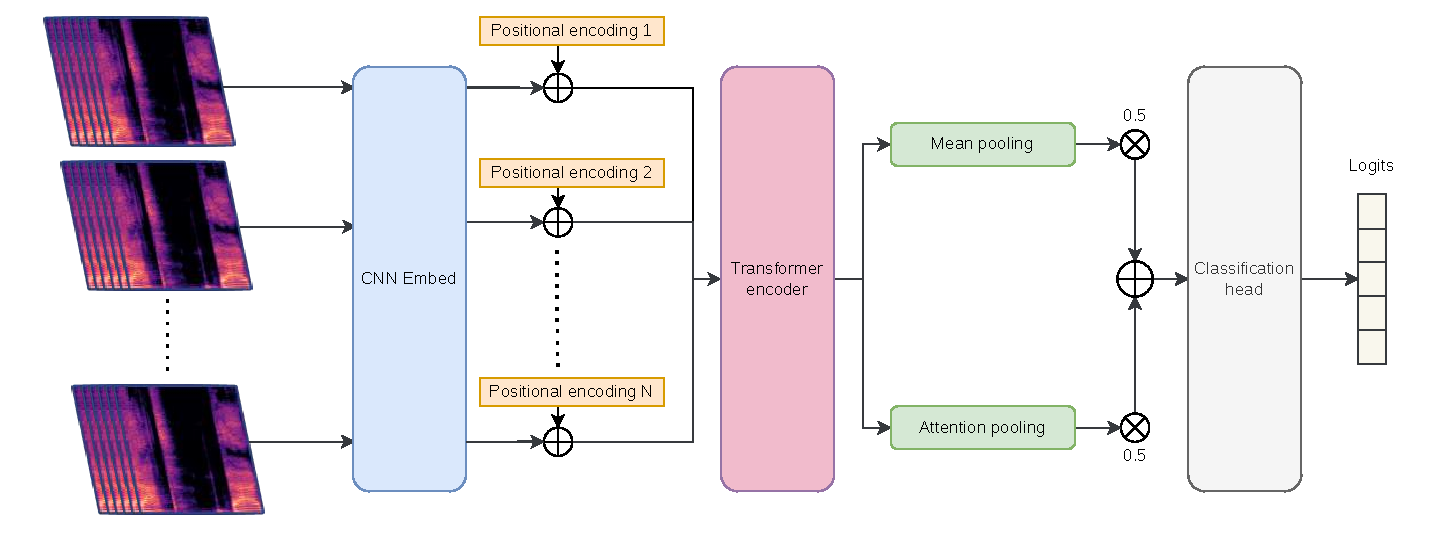
\includegraphics[width=1\linewidth]{models/baseline.drawio.pdf}
    \end{center}
\caption{Baseline model architecture.}
\label{baseline_model_architecture}
\end{figure}

The model consists of two main components: 
\begin{itemize}
    \item A feature extractor, implemented using a convolutional neural network (CNN) architecture, which gets a single epoch as an input,
    \item and a classifier, implemented using a transformer encoder, which predicts the sleep stage based on the embeddings extracted by the feature extractor.
\end{itemize}

\subsubsection*{Feature Extraction}
The feature extractor receives a single epoch (represented as a spectrogram image per EEG channel) as an input and outputs an embedding (array of numbers, representing the learned features of the epoch).
The CNN module consists of two sequential 2D convolutional blocks. Each block utilizes $3 \times 3$ kernels with a stride of 2,
followed by a ReLU activation function and Group Normalization to stabilize training without relying on batch statistics.
The output feature maps are flattened, subjected to Dropout (to mitigate overfitting), and passed through a linear projection layer to
produce a fixed-size token for each epoch.

\subsubsection*{Sequence Modeling and Contextualization}
Because sleep stages are not independent, analyzing epochs in isolation is suboptimal.
Therefore, the network processes a contextual window of 10 consecutive epochs with the goal of predicting the sleep stage of the central epoch.
Each epoch's token has an added learned positional embedding to retain temporal information, allowing the model to understand the order of epochs within the sequence.
These tokens are then passed into a standard Transformer Encoder.
The self-attention mechanism allows the model to weigh the importance of surrounding epochs when evaluating the central epoch.

To aggregate the sequence of contextualized tokens into a single representation for classification, we employ a hybrid pooling strategy. The final representation is an unweighted average of two techniques:
\begin{enumerate}
\item \textbf{Mean Pooling:} The average of all token embeddings across the temporal dimension.
\item \textbf{Attention Pooling:} A learned linear layer projects the tokens to compute raw attention scores. These scores are 
normalized across the temporal dimension using a Softmax function, 
producing weights that sum to one. The pooled representation is the weighted sum (using the computed weights) of the sequence tokens.
\end{enumerate}

Finally, this aggregated representation is passed through a classification head—a multilayer perceptron (MLP) consisting of a linear layer, a ReLU activation, Dropout, and a final linear layer—yielding the logits for the 5 sleep stages.
During training the loss is calculated on the central token using Focal Loss, which is particularly effective for handling class imbalance by down-weighting easy examples and focusing on harder, misclassified examples.

\subsection{Model with additional embeddings} \label{sec:additional_embeddings}

To explicitly account for the age-related domain shifts established in Section \ref{sec:motivation}, we developed a secondary architecture designed to actively integrate patient age metadata into the sequence modeling process.

\begin{figure}
    \begin{center}
        \includegraphics[width=1\linewidth]{models/embeddings.drawio.pdf}
    \end{center}
\caption{Model with additional embeddings.}
\label{embeddings_model_architecture}
\end{figure}

\subsubsection*{Feature Extraction}
The spatial-frequency feature extraction phase of this model is identical to the baseline. The input consisting of 10 consecutive 30-second epochs is passed through the Convolutional Neural Network (CNN) module, producing a sequence of 10 dense feature vectors (tokens).

\subsubsection*{Metadata Integration via a Learnable Class Token}
The primary divergence from the baseline model lies in how the sequence is contextualized. Inspired by architectures such as BERT and ViT, we introduce a learnable classification token (\texttt{[CLS]}). This token acts as a global placeholder that accumulates sequence-wide context during the Transformer's self-attention operations.

To inject the demographic data into the model, the patient's age is first discretized into one of 4 categorical age groups:
\begin{itemize}
    \item infant (0--2 years),
    \item child (2--12 years),
    \item teen (13--18 years),
    \item adult (19+ years).
\end{itemize}

This categorical value is passed through an embedding layer, mapping the age group to a dense vector of the same dimensionality as the EEG tokens. 
Instead of concatenating this metadata to every epoch, the age embedding is combined with the expanded \texttt{[CLS]} token via element-wise addition. Consequently, the \texttt{[CLS]} token becomes an ``age-aware'' global summary token before any sequence processing begins.

\subsubsection*{Sequence Modeling and Representation Extraction}
Once the age-aware \texttt{[CLS]} token is formulated, it is prepended to the sequence of 10 EEG tokens, expanding the overall sequence length to 11. Because the sequence length has increased, the learned positional embedding space is also expanded to 11. These positional embeddings are added to all tokens to establish chronological order, and the combined sequence is fed into the Transformer Encoder.

Unlike the baseline model, which employed a hybrid strategy of Mean and Attention pooling across all epoch tokens to derive a final representation, this updated architecture utilizes a much simpler extraction paradigm. The self-attention mechanism within the Transformer naturally routes relevant temporal and spatial information from the EEG tokens into the prepended \texttt{[CLS]} token. Therefore, upon exiting the Transformer, we discard the 10 epoch tokens and extract only the contextualized \texttt{[CLS]} token.

This single token, which now encapsulates both the contextualized EEG sequence data and the patient's age profile, serves as the definitive global representation. It is passed directly into the MLP classification head to generate the final sleep stage logits.
\subsubsection*{Demographic Batch Balancing}
To ensure the model effectively learns to utilize this age profile across all demographics, we had to address a significant imbalance in the training data. Because adult recordings vastly outnumber pediatric and infant recordings, standard random sampling would bias the network toward adult EEG patterns, severely limiting its ability to learn accurate representations for the younger age cohorts. Therefore, a class-balanced weighted sampling strategy was introduced during the training phase. By assigning sampling probabilities that were inversely proportional to the total number of epochs available for each of the four age groups, we guaranteed that every training batch contained a demographically balanced distribution of data.

\subsection{Separate models (Age-Stratified Framework)} \label{sec:separate_models}

In our third experimental approach, we explore an alternative method for handling demographic variance. Rather than relying on a single, generalized network to learn the complexities of age-related EEG shifts (as attempted in the embedding-based model), we hypothesized that isolating the training data distributions might yield superior results. To test this, we developed an age-stratified routing framework.

\begin{figure}
    \begin{center}
        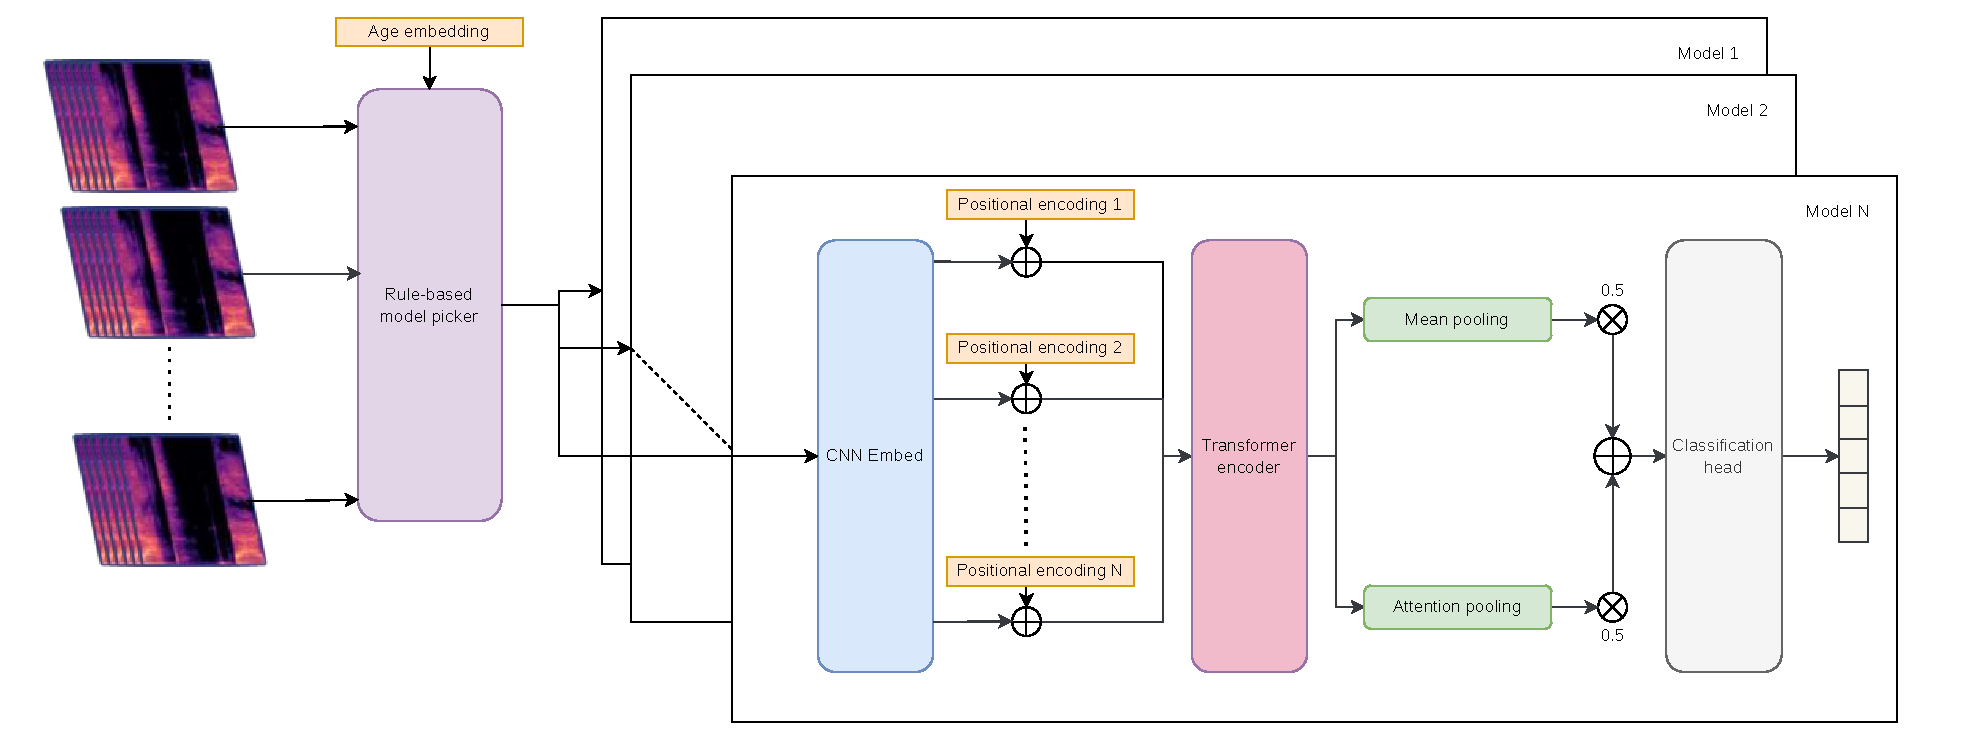
\includegraphics[width=1\linewidth]{models/seperate models.drawio.pdf}
    \end{center}
\caption{Separate trained models per patient metadata.}
\label{embeddings_model_architecture}
\end{figure}

\subsubsection*{Architecture and Data Partitioning}
For this framework, the neural network architecture reverts entirely to the original Baseline model. 
Instead of altering the model's internal architecture, we altered the training data distribution.
The global training dataset was partitioned into four age groups defined in previous section.

We independently initialized and trained four distinct instances of the baseline model, one for each demographic cohort. Consequently, each model acts as a demographic expert, highly specialized in the specific characteristics of its respective age group.

\subsection{Fine-tuned model} \label{sec:finetuning}
In our fourth and final experimental approach, we explore a transfer
learning paradigm. Typically, in physiological datasets, data from
adult cohorts is vastly more abundant than data from pediatric or
infant cohorts. To leverage this imbalance, we hypothesized that a model
could first learn foundational, universal EEG characteristics from
the largest demographic group and later learn age-specific patterns
on smaller specific datasets.

The foundation of this framework is the adult specific model from 
section \ref{sec:separate_models}.
We prepare the trained model for fine-tuning on the remaining age groups (infants, children, and teens). Rather than updating the entire network during fine-tuning—which risks catastrophic forgetting and overfitting on smaller pediatric cohorts—we employ a selective partial layer-freezing strategy. 

Specifically, the gradient updates are configured as follows:
\begin{itemize}
    \item \textbf{Frozen Feature Extractor:} The parameters of the Convolutional Neural Network are completely frozen. The underlying assumption is that low-level spectrogram features extracted by the CNN are similar across all ages. Freezing this module preserves these generalized feature representations.
    \item \textbf{Unfrozen Sequence Modeling:} The Transformer encoder layers are unfrozen. While low-level EEG features may be universal, the temporal dynamics of sleep, such as the duration of sleep cycles, and transition probabilities, change significantly from infancy to adulthood. Unfreezing the Transformer allows the self-attention mechanism to adapt to these age-specific sequential patterns.
    \item \textbf{Unfrozen Classification Head:} The final MLP mapping the pooled representation to the 5 sleep stages is also unfrozen. This ensures the decision boundaries can shift to accommodate the updated temporal representations.
\end{itemize}

This approach acts as a hybrid between the generalized Baseline model and the specialized framework. By isolating the layers responsible for temporal context and classification, this framework aims to retain the robust, generalized feature-extraction capabilities learned from a massive adult dataset, while adapting only the reasoning modules to other age groups.